\modeCorrection

%%%% Définition En-tête et pied de page 
\pagestyle{fancy}
\renewcommand\footrulewidth{1pt}
\fancyhead[L]{Devoir commun de Physique-Chimie}
\fancyhead[R]{Lycée Parc de Vilgénis}
\fancyfoot[C]{\textbf{Page \thepage/\pageref{LastPage}}}

\renewcommand{\thesubsection}{\textcolor{red}{\Roman{section}.\arabic{subsection}}}
\renewcommand{\thesubsubsection}{\textcolor{red}{\Roman{section}.\arabic{subsection}.\alph{subsubsection}}}
\renewcommand{\titreDocu}[1]{
  \refstepcounter{document} % update counter
  \textbf{Exercice \arabic{document} -- #1} 
  \addcontentsline{toc}{document}{\protect\numberline{} #1} % update table of content
}


\renewcommand{\numeroQuestion}{
  \refstepcounter{exercice}
  \vspace*{2pt}
  \hspace{15pt}
  \textcolor{black}{%couleurPrincipale!75!black}{
    \textbf{Q.\arabic{exercice}}
  }
}

\setcounter{section}{0}
\setcounter{document}{0}


%\nomPrenomClasse
\vspace{1cm}

\begin{center}
\begin{Huge}
    DEVOIR COMMUN DE SECONDE
\end{Huge}
\end{center}
\vspace{1cm}

\vspace{1cm}

\begin{center}
    \begin{large}
        Jeudi 21 Décembre 2023
    \end{large}
\end{center}

\vspace{2cm}

\begin{center}
    \begin{Large}
        \textbf{PHYSIQUE-CHIMIE}\\
    \end{Large}
\end{center}
\vspace{2cm}


\begin{center}
    \begin{large}
        Durée de l'épreuve : \textbf{2 heures}\\
    \end{large}
\end{center}
\vspace{1cm}
\begin{center}
    \begin{large}
        \textit{L'usage de la calculatrice est autorisé.}\\
    \end{large}
\end{center}
\vspace{1cm}
\begin{center}
    \begin{large}
        Dès que ce sujet vous est remis, assurez-vous qu’il est complet.\\
        Ce sujet comporte \pageref{LastPage} pages numérotées de \thepage/\pageref{LastPage} à \pageref{LastPage}/\pageref{LastPage}.
    \end{large}
\end{center}

\begin{tcolorbox}[colback=red!5!white,colframe=red!75!black,title=\textbf{Consignes : }]
   \begin{enumerate}
       \item Pour les élèves bénéficiant d'un tiers-temps, vous ne traiterez pas les questions marquées par $(*)$ ; 
       \item Lisez-bien l'énoncé des exercices. Les questions sont pour la plupart indépendantes. Si vous bloquez sur une question, passez à la suivante ;
       \item N'oubliez pas d'encadrer ou de souligner vos résultats ;
       \item Vous rendrez l'énoncé avec la copie.
   \end{enumerate}
\end{tcolorbox}
\newpage

%\begin{tableauCompetences}
%    APP & S'approprier les informations d'un document & & & & \\
%    \hline
%    REA & Utiliser les pourcentages et les fractions  & & & & \\
%     \hline 
%    ANA &  Exploiter les informations extraites des données & & & & \\
%    \hline
%    VAL & Valider/critiquer un modèle & & & &
%\end{tableauCompetences}



\begin{doc}{Le gaz de ville \begin{large}
    /9 points
\end{large}}
\vspace{-0.4cm}
\begin{wrapfigure}{r}{0.35\textwidth}
\vspace{-0cm}
    \centering
      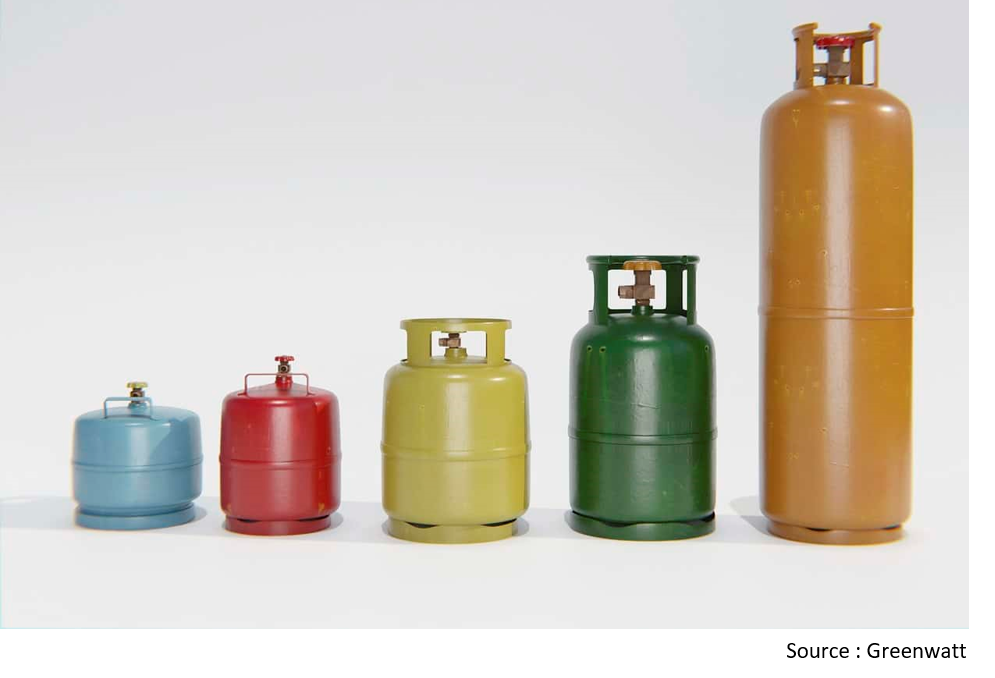
\includegraphics[scale=0.35]{Images/DS/Devoir_Commun/Bouteille_gaz.png}
  \end{wrapfigure}
L'odeur de gaz vous est désagréable, mais c'est pour votre bien ! Le saviez-vous ?\\
Le gaz de ville, celui qui arrive dans les habitations par des tuyaux de distribution collective, est principalement constitué de méthane. Le méthane est incolore et inodore, mais alors d'où vient l'odeur si caractéristique du gaz de ville ?\\
Ce que l'on appelle « odeur de gaz » est en réalité dû à un additif ajouté, le tétrahydrothiophène (THT), pour rendre les fuites de gaz détectables et prévenir du danger qu’elles représentent. En effet, le méthane devient fortement explosif lorsqu'il atteint une certaine concentration dans l'air.\\

On considère une bouteille de gaz de ville de volume $V=100$~L. L’étiquette sur la bouteille indique le pourcentage volumique des deux espèces chimiques présentes dans ce mélange :

\begin{center}
    \begin{tabular}{|C{0.45}|C{0.45}|}
        \hline
        \multicolumn{2}{|c|}{\cellcolor{blue!25}Composition du mélange contenu dans la bouteille de gaz de ville} \\
        \hline
        \cellcolor{orange!25}Nom de la substance & \cellcolor{orange!25}Pourcentage volumique \\
        \hline
        tétrahydrothiophène (THT) & 0,10225 \% \\
        \hline 
         Méthane & 99,89775 \%  \\
         \hline
    \end{tabular}
\end{center}
Voici quelques données sur le méthane :
\begin{center}
    \begin{tabular}{|c|C{0.3}|}
        \hline
        \cellcolor{orange!25}Pictogrammes de sécurité du méthane &
            
\includegraphics[scale=0.3]{Images/DS/Devoir_Commun/Picto.png}
         \\
        \hline
        \cellcolor{orange!25}Température de fusion (en $\degreCelsius$) à la pression atmosphérique & $-182,47$ \\
        \hline
        \cellcolor{orange!25}Température d'ébullition (en $\degreCelsius$) à la pression atmosphérique & $-161,52$ \\
        \hline 
        \cellcolor{orange!25}Masse volumique du méthane (en g$\cdot$L$^{-1}$) & 0,657 \\
         \hline
    \end{tabular}
\end{center}


\question{Rappeler la définition d’un mélange et proposer un exemple. (1pt)}{Un mélange est constitué de plusieurs espèces chimiques (0,5pt). Exemple : la vinaigrette, le sang, l'air, etc. (0,5pt).}{0}
\\
\vspace{-0.2cm}
\question{Il est conseillé de ne pas conserver une bouteille de méthane à proximité d’une fenêtre exposée au soleil. Justifier à l’aide des pictogrammes de sécurité du méthane.(1pt)
}{Le pictogramme 
\includegraphics[scale=0.08]{Images/Methodo/Fiche_Methode1/SGH02_Flamme.jpg} indique inflammable (1pt). Il faut donc le protéger des sources de chaleur possible (comme le soleil derrière une fenêtre qui fait loupe).}{0}
\\
\vspace{-0.2cm}
\question{Indiquer l’état physique du méthane à température ambiante (20°C) et à la pression atmosphérique. Justifier. (1pt)}{Les températures d'ébullition et de fusion sont bien plus basses que la température ambiante d'après les données de l'énoncé. Le méthane est donc gazeux à la température $T=20\degreCelsius$.}{0}
\\
\vspace{-0.2cm}
\question{\`{A} l’aide des documents, déterminer le volume de chaque espèce chimique présente dans la bouteille de gaz de ville. (2pts)}{D'après la définition de la proportion volumique $x_{v}$, $x_{v,\text{espèce}}=\frac{V_{\text{espèce}}}{V}$ (1pt). On en déduit :
\begin{align*}
    V_{\text{méthane}} &= V\times x_{v,\text{méthane}} = 100\times\frac{99,89775}{100} = 99,89775~\text{L (0,5pt)} \\
    V_{\text{THT}} &= V\times x_{v,\text{THT}} = 100\times\frac{0,10225}{100} = 0,10225~\text{L (0,5pt)}
\end{align*}}{0}
%\newpage%\\
\question{$(*)$ En déduire la masse de méthane $m_{\text{méthane}}$ contenue dans la bouteille. (1pt)}{D'après la définition de la masse volumique $\rho = \frac{m}{V}$ (0,5pt), on en déduit $m_{\text{méthane}}$ : 
\begin{align*}
    m_{\text{méthane}} &= \rho_{\text{méthane}}\times V \\
     &= 0,657 \times 99,89775 = 65,6~\text{g (0,5pt)}
\end{align*}}{0}
\\
Voici un graphe donnant la masse volumique du mélange méthane/THT en fonction du pourcentage volumique du THT dans le mélange : 
\begin{center}
    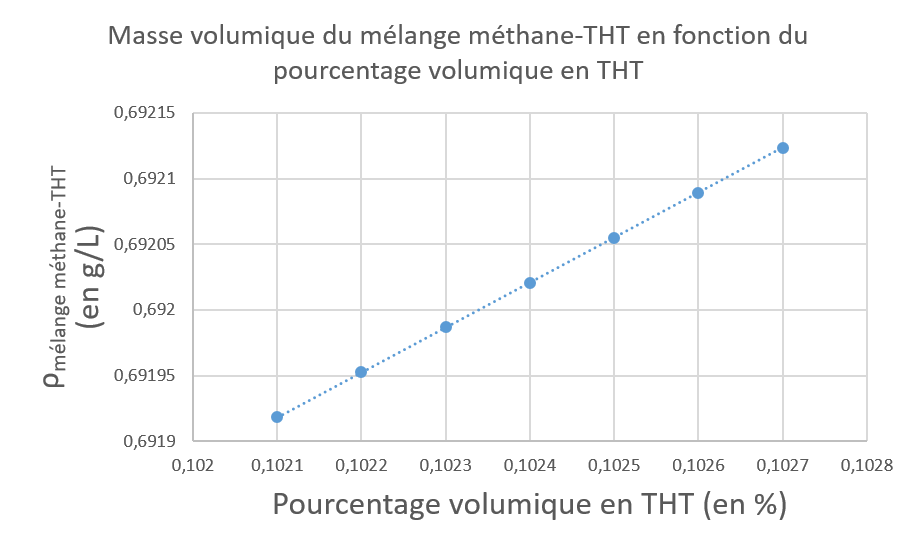
\includegraphics[scale=1]{Images/DS/Devoir_Commun/Graphe_rhovspourcentagevol.png}
\end{center}
\question{Déterminer graphiquement la masse volumique du mélange $\rho_{\text{mélange}}$ dans la bouteille de gaz de ville. Vous ferez apparaître la construction sur le graphique. (1pt)}{\begin{center}
    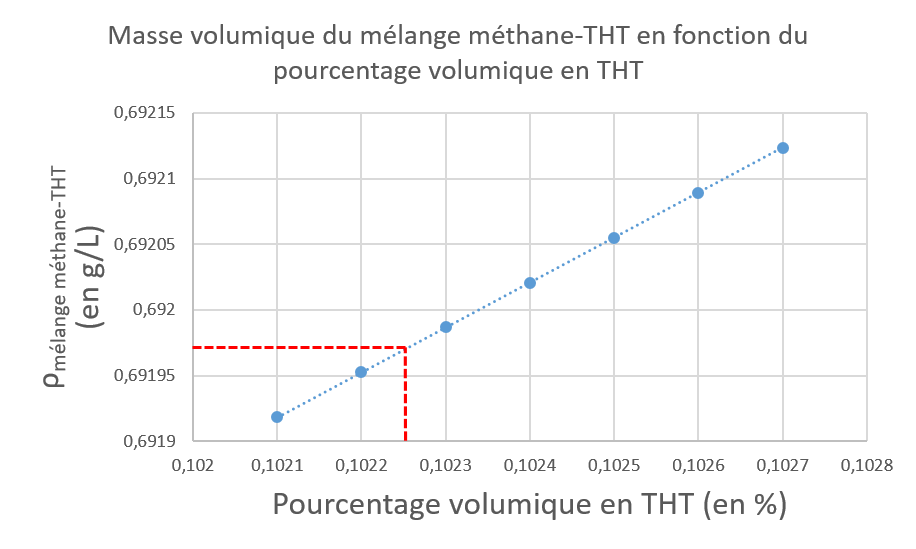
\includegraphics[scale=1]{Images/DS/Devoir_Commun/Graphe_rhovspourcentagevol_correction.png}
\end{center}
\textcolor{red}{On trouve $\rho_{\text{mélange}}=0,69197$~g.L$^{-1}$ (0,5pt pour la construction graphique, 0,5pt pour le résultat)%($\rho_{\text{mélange}}=0,69198$~g.L$^{-1}$ acceptée.)
}}{0}
\\
\textbf{Pour la question suivante, toute tentative de réponse même non aboutie sera valorisée.}\\
\question{$(*)$ La norme imposée au gaz de ville est qu’il doit contenir entre $15$~mg et $40$~mg de THT par litre de gaz. Exprimer la masse volumique du mélange en fonction de la masse des espèces chimiques et du volume de la bouteille. En déduire la masse de THT présente dans la bouteille de gaz étudiée. Respecte-t-elle la norme imposée au gaz de ville ? Justifier en rédigeant une réponse scientifiquement argumentée. (2pts)}{On part de : 
\begin{equation*}
    \rho_{\text{mélange}} = \frac{m_{\text{mélange}}}{V} = \frac{m_{\text{méthane}}+m_{\text{THT}}}{V}~\text{(1pt)}
\end{equation*}
On isole $m_{\text{THT}}$ :
\begin{align*}
    \frac{m_{\text{THT}}}{V} &= \rho_{\text{mélange}} - \frac{m_{\text{méthane}}}{V} \\
    m_{\text{THT}} &= V\times \left(\rho_{\text{mélange}} - \frac{m_{\text{méthane}}}{V} \right)~\text{(0,5pt)}\\
    m_{\text{THT}} &= 100\times \left(\rho_{0,69197} - \frac{65,7}{100}\right) = 35,0~\text{mg (0,5pt)}
\end{align*}}{0}
%\\
\end{doc}

%%%%%%%%%%%%%%%%%%%%%%%%%%%%%%%%%
\newpage
%%%%%%%%%%%%%%%%%%%%%%%%%%%%%%%%%
\setcounter{exercice}{0}
\begin{doc}{Solutions aqueuses \begin{Large}
    /9 points
\end{Large}}
\begin{wrapfigure}{r}{0.3\textwidth}
\vspace{-1cm}
    \centering
      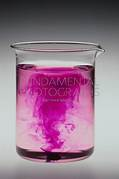
\includegraphics[scale=1.0]{Images/DS/Devoir_Commun/Permanganate.png}
  \end{wrapfigure}
\og Le permanganate de potassium est un solide gris-violet de formule \chemform{KMnO_4}. Dissous dans l’eau, il donne des solutions de couleur violette.\\
Pour soigner les érythèmes (irritations de la peau), il est recommandé d’utiliser des solutions aqueuses de permanganate de potassium de concentration en masse égale à $0,10$~g$\cdot$L$^{-1}$.\\
En solution aqueuse à $0,50$~g$\cdot$L$^{-1}$, le permanganate de potassium est également utilisé comme désinfectant pour laver les légumes dans les pays tropicaux.\fg
\begin{flushright}
    \textit{D’après le site \url{ societechimiquedefrance.fr/permanganate-de-potassium}}.
\end{flushright}

L’objectif de l’exercice est d’estimer la concentration d’une solution aqueuse S de permanganate de potassium afin de valider ou non son utilisation pour soigner les érythèmes ou pour laver les légumes.\\

Pour cela, on prépare 250 mL d’une solution aqueuse S$_0$ de permanganate de potassium de concentration en masse $C_{m,0} = 0,60$~g$\cdot$L$^{-1}$ en dissolvant dans l’eau une masse appropriée de permanganate de potassium solide.\\


\question{Identifier le solvant et le soluté des solutions utilisées pour soigner les érythèmes ou pour laver les légumes. (1pt)}{Solvant : eau (0,5pt), soluté : \chemform{KMnO_4} (0,5pt).}{0}
\\
\question{$(*)$ Donner le nom de la technique utilisée pour préparer la solution S$_0$. (0,5pt)}{Il s'agit d'une dissolution.}{0}
\\
\question{Donner l’expression de la concentration en masse $C_m$ d’une solution en fonction de la masse de soluté $m_{\text{soluté}}$ et du volume de solution $V_{\text{solution}}$. (0,5pt)}{$C_m = \frac{m_{\text{soluté}}}{V_{\text{solution}}}$}{0}
\\
\question{En déduire la valeur de la masse de permanganate de potassium qui a été dissoute pour préparer 250 mL de solution S$_0$. (1,5pts)}{L'énoncé annonce $V_{\text{solution}}=250$~mL et $C_{m,0} = 0,60$~g$\cdot$L$^{-1}$, on en déduit :
\begin{align*}
    m_{\text{\chemform{KMnO_4}}} &=C_{m,0}\times V_{\text{solution}}~\text{( 0,5pt)} \\
    &= 0,60\times0,250 = 0,15~\text{g  (0,5pt calcul + 0,5pt unités)}
\end{align*}}{0}
%\\

\newpage
On prépare ensuite cinq solutions S$_1$, S$_2$, S$_3$, S$_4$ et S$_5$ en prélevant différents volumes de solution aqueuse S$_0$ de permanganate de potassium de concentration en masse $C_{m,0} = 0,60$~g$\cdot$L$^{-1}$ et en y ajoutant de l’eau distillée pour obtenir un volume de 50,0 mL de solution (voir tableau ci-après).
\begin{center}
    \begin{tabular}{|C{0.1}|C{0.2}|C{0.2}|C{0.3}|}
        \hline
        \cellcolor{blue!25}Solution & \cellcolor{blue!25}Volume de solution S$_0$ à prélever (mL) & \cellcolor{blue!25}Volume de solution obtenue (mL) & \cellcolor{blue!25}Concentration en masse de la solution obtenue (g$\cdot$L$^{-1}$) \\
        \hline 
        S$_1$ & 2 & 50,0 & 0,024 \\
        \hline
        S$_2$ & 5 & 50,0 & 0,060 \\
        \hline
        S$_3$ & 10 & 50,0 & 0,12 \\
        \hline
        S$_4$ & 15 & 50,0 & 0,18 \\
        \hline
        S$_5$ & ~? & 50,0 & 0,24 \\
        \hline
    \end{tabular}
\end{center}

\question{Donner le nom de la technique utilisée pour préparer les cinq solutions S$_1$, S$_2$, S$_3$, S$_4$ et S$_5$. (0,5pt)}{Il s'agit d'une dilution.}{0}
\\
\question{Écrire le protocole expérimental qui a été suivi pour préparer 50,0 mL de solution S$_1$. Préciser soigneusement le nom du matériel utilisé. (1,5pts)}{\begin{enumerate}
\item On prélève un volume $V_{\text{prélevé}}$ de solution S$_0$ à l'aide d'une pipette jaugée et d'une propipette (0,5pt pour pipette jaugée);
\item On verse le volume prélevé dans une fiole jaugée de 50,0~mL (0,5pt pour la fiole) ;
\item On remplit la fiole jaugée au 2/3 avec de l'eau distillée et on agite ;
\item On complète jusqu'au trait de jauge avec une pipette pasteur pour faire coïncider le trait de jauge avec le bas du ménisque (0,5pt le ménisque) ;
\item On bouche la fiole avec un bouchon et on agite ;
\end{enumerate}}{0}
%\\
\question{Déterminer la valeur du volume de solution S$_0$ qui a été prélevé pour préparer 50,0 mL de solution S$_5$. Justifier précisément le calcul effectué. (2pts)}{D'après le loi de conservation de la masse de soluté prélévé au cours de la dilution :
\begin{align*}
   C_{m,0} \times V_{\text{prélevé}} &= C_{m,S_5}\times V_{fille}~\text{( 0,5pt)}\\
    V_{\text{prélevé}} &=\frac{C_{m,S_5}V_{fille}} {C_{m,0}}~\text{( 0,5pt)}\\
    &= \frac{0,24\times0,05}{0,60} = 20~\text{mL}~\text{( 0,5pt pour le calcul + 0,5pt pour les unités)}
\end{align*}}{0}
%\\
On verse les cinq solutions S$_1$, S$_2$, S$_3$, S$_4$ et S$_5$ dans des tubes à essais : on obtient ainsi une échelle de teintes (voir photo ci-dessous).
\begin{center}
    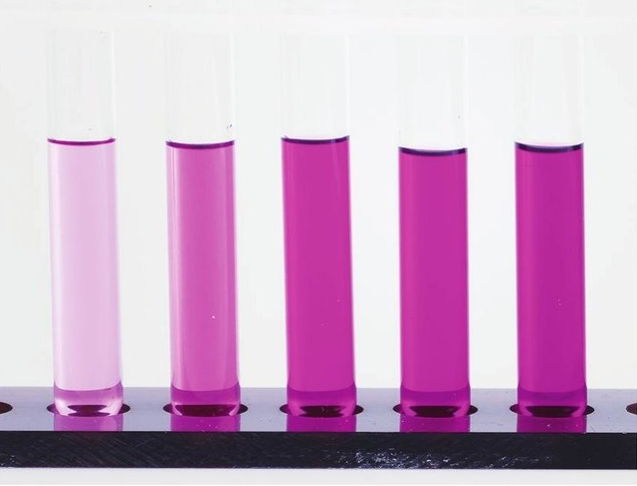
\includegraphics[scale=0.5]{Images/DS/Devoir_Commun/Echelle_teinte.png}
\end{center}
On verse ensuite la solution S dans un sixième tube à essais. On constate que la teinte de la solution S est comprise entre celles des solutions S$_2$ et S$_3$.\\
\question{Déterminer un encadrement de la concentration en masse de la solution S. (1pt)}{$0,060~\text{g$\cdot$L$^{-1}$}<C_{m,0}<0,12~\text{g$\cdot$L$^{-1}$}$}{0}
\\
\question{$(*)$ En déduire si la solution $S$ peut être utilisée pour soigner les érythèmes ou pour laver les légumes. Justifier.(0,5pt)}{Une réponse possible : comme on n'est pas sur que la concentration soit égale à 10~g$\cdot$L$^{-1}$, on ne peut pas utiliser la solution pour soigner les érythèmes. (0,5pt en reprenant l'énoncé et en faisant un raisonnement logique).}{0}
\end{doc}
\setcounter{exercice}{0}
\begin{doc}{Le son d’une guitare
 \begin{Large}
    /12 points
\end{Large}}
Une guitare se compose d'un coffre auquel est accroché un manche sur lequel sont tendues des cordes métalliques ou en nylon. La photo ci-dessous présente une guitare ainsi qu'un zoom sur une partie du manche après avoir frotté les cordes :

\begin{center}
    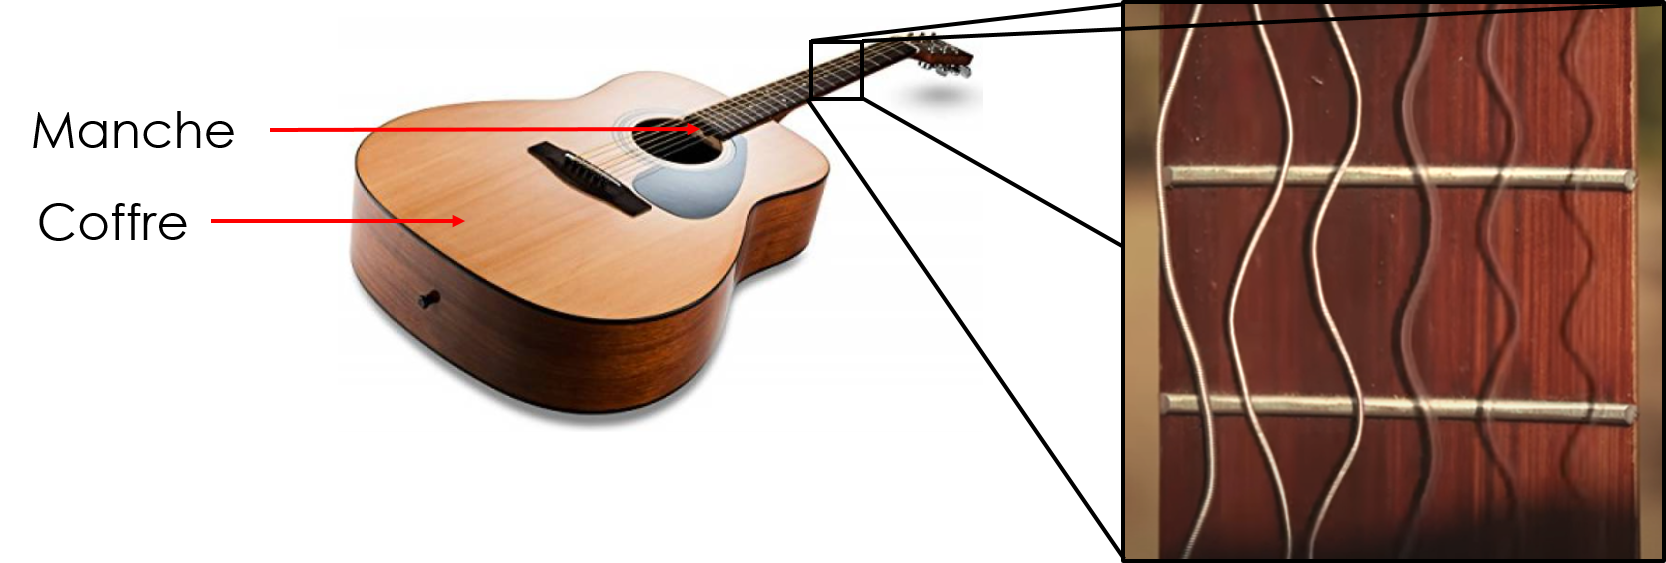
\includegraphics[scale=0.5]{Images/DS/Devoir_Commun/Guitare.png}
\end{center}

Voici un tableau des notes (do, ré, mi, fa, sol, la, si) et des fréquences (en Hz) correspondantes de la gamme tempérée :
\begin{center}
    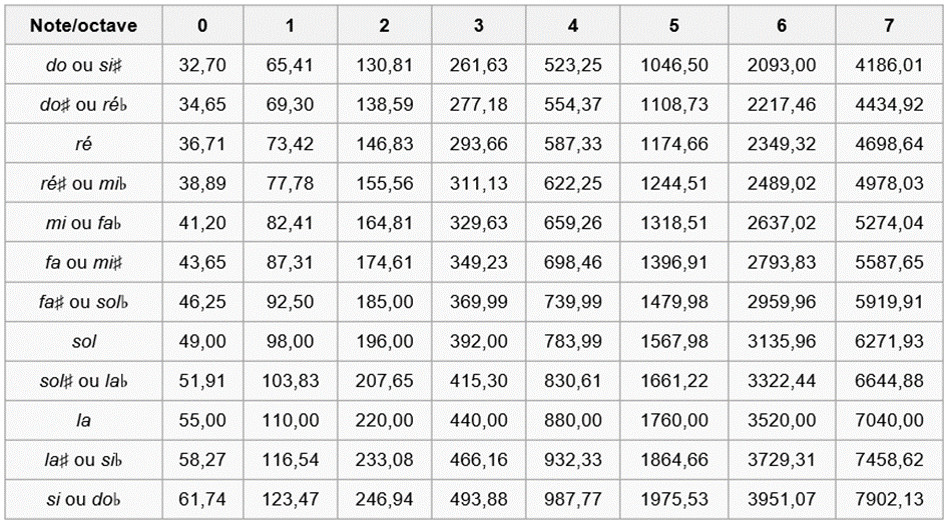
\includegraphics[scale=0.7]{Images/DS/Devoir_Commun/Notes_guitare.png}
\end{center}

On dit qu'une note est jouée \og à vide \fg~ lorsqu'on laisse la corde de guitare vibrer librement sur toute sa longueur. De la corde la plus épaisse à la plus fine, les six notes jouées à vide sont : \og mi2, la2, ré3, sol3, si3, mi4 \fg~.
\newpage
\question{Indiquer l'origine du son émis par une guitare. (1pt)}{Les cordes vibrent et font vibrer les molécules d'air de proche en proche. (1pt) La vibration va être perceptible par notre tympan qui va nous faire entendre un son.}{0}
\\
\question{Donner l'intérêt physique du coffre d'une guitare. (1pt)}{Le coffre sert de caisse de résonance, c'est-à-dire qu'il sélectionne et amplifie (1pt pour amplifie) le son émis par le frottement des cordes de guitare.}{0}
\\
\question{Indiquer la condition pour que le son se propage dans un milieu. (0,5pt)}{Il faut un milieu matériel pour que le son puisse se propager.}{0}
%\\
\question{Identifier le milieu dans lequel le son se propage de la guitare jusqu'à notre oreille puis rappeler la valeur de la vitesse de propagation du son dans ce milieu. (1pt)}{Ici, le milieu est l'air (0,5t) et la vitesse vaut (à $15\degreCelsius$) 340~m$\cdot$s$^{-1}$ (0,5pt).}{0}
\\
\question{Calculer la durée $\Delta t$ que met le son à se propager jusqu’à l’auditeur lorsqu'il se trouve à une distance d=1km. (2pts). \textit{(Bonus) : l'auditeur parviendre-t'il a entendre ce son ? Justifier. (1pt)}}{
\begin{align*}
    v_{son} &= \frac{d}{\Delta t} ~\text{(0,5pt)}\\
    \Delta t &= \frac{d}{v_{son}} ~\text{(0,5pt)}\\
             &= \frac{1000}{340} = 2,94~\text{s (0,5pt calcul + 0,5pt unités)}
\end{align*}
L'auditeur ne parviendra sans doute pas à entendre car le son s'atténue avec la distance.}{0}

%\\
\question{$(*)$ Donner le domaine des fréquences audibles pour un être humain. (1pt)}{Entre 20~Hz et 20000~Hz.}{0}
\\
\question{Un chat est capable d’entendre des fréquences comprises entre 20 Hz et 60 kHz. Peut-il entendre la note la plus grave jouée avec une guitare ? Justifier la réponse. (1pt)}{Oui car la note la plus grave sonne à la fréquence 32,70~Hz qui est comprise dans le domaine de fréquence audible du chat.}{0}
\\
\question{$(*)$ Donner les valeurs des fréquences des 6 notes jouées à vides à la guitare. (1,5pts)}{0,5pt pour deux bonnes réponses :\begin{itemize}
    \item mi2 : $f_{mi2}=164,81$~Hz ;
    \item la2 : $f_{la2}=220,00$~Hz ;
    \item ré3 : $f_{ré3}=293,66$~Hz ;
    \item sol3 : $f_{sol3}=392,00$~Hz ;
    \item si3 : $f_{si3}=493,88$~Hz ;
    \item \textcolor{red}{mi4 : $f_{mi4}=659,26$~Hz };
\end{itemize}}{0}
%\\
\question{Entre la note mi2 et la note mi3, donner le son le plus aigu. Justifier.(1pt)}{Il s'agit de la note mi3 (0,5pt) car elle possède la fréquence la plus haute (0,5pt).}{0}
\\
Un ingénieur du son a enregistré une note émise par une guitare, à l’aide d’un microphone relié à un système informatisé. Voici le signal enregistré :
\begin{center}
    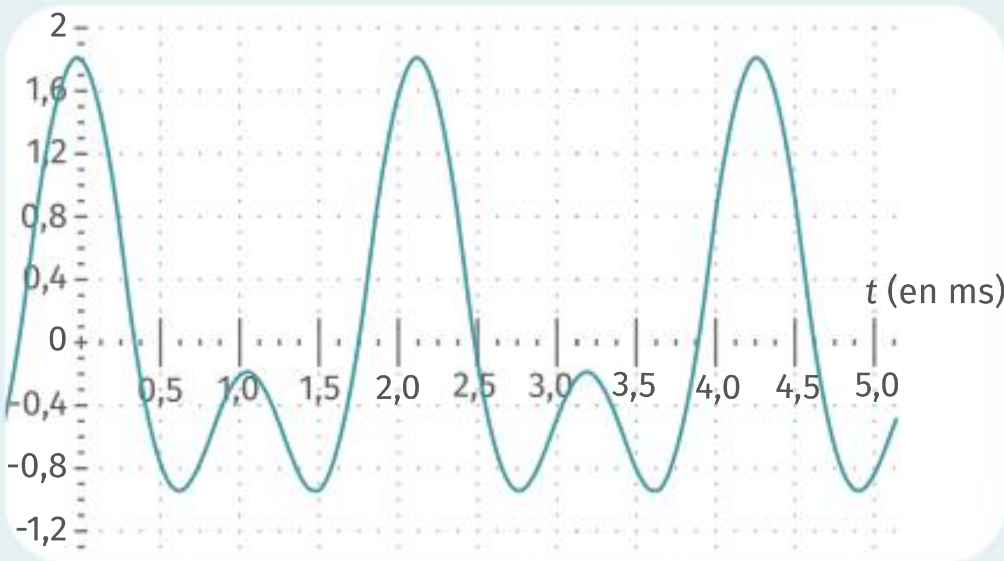
\includegraphics[scale=0.5]{Images/DS/Devoir_Commun/Signal_guitare.PNG}
\end{center}
\question{Donner la formule reliant la fréquence $f$ et la période $T$ d’un signal. Déterminer la fréquence $f$ de la note émise par la guitare. (2pts)}{$f=\frac{1}{T}~\text{(0,5pt)} = \frac{1}{2,13\times 10^{-3}}~\text{(1pt)}=470$~Hz (0,5pt).}{0}

\end{doc}
\vspace{2cm}
\begin{center}
\begin{Huge}
    \textbf{FIN DU SUJET.}
\end{Huge}
\end{center}